\documentclass[11pt]{article}
\usepackage[margin=1in]{geometry}
\usepackage{booktabs,graphicx,amsmath,caption,hyperref,setspace}
\usepackage[round]{natbib}
\hypersetup{colorlinks=true,linkcolor=black,citecolor=black,urlcolor=blue}
\captionsetup{font=small,labelfont=bf}
\setstretch{1.1}
\graphicspath{{../output/figures/}}

\title{Who Ran on USDC? Wallet-Level Evidence from\\ the March 2023 Stablecoin Depeg}
\author{Kunjian Li\thanks{Independent research note. All data are extracted directly from the Ethereum blockchain; code is available in the accompanying repository.}}
\date{\today}

\begin{document}
\sloppy
\maketitle

\begin{abstract}
\noindent When Silicon Valley Bank failed on March 10, 2023, Circle disclosed that \$3.3 billion of USDC reserves were held there and USDC traded as low as \$0.883. I reconstruct every USDC transfer on Ethereum from March 1 to March 20, 2023 (1.92 million transfers, 493,077 addresses) directly from blockchain event logs, and validate the data against on-chain state: issuance net of redemptions matches the change in token supply to the cent. Three patterns emerge. First, the primary market contracted sharply: \$5.2 billion of USDC was burned during the four-day stress window while issuance nearly stopped over the weekend, and \$2.1 billion flowed into MakerDAO's Peg Stability Module, where USDC could be swapped for DAI at par. Second, on-chain activity broadened rather than concentrated: daily active senders rose fourfold and the share of outgoing volume from the top 100 senders fell from about 85\% to 48\%. Third, comparing each wallet's behavior during the stress window with a placebo window one week earlier, smaller holders were much more likely to exit: 63\% of wallets holding \$1k--\$10k moved out at least half their balance, compared with 36\% of wallets holding over \$10 million. The pattern is consistent with large holders relying on primary-market redemption rather than selling on-chain at a discount, a hypothesis I outline for further work.
\end{abstract}

\section{Introduction}

Stablecoins are run-prone by design: they promise par convertibility while investing reserves in assets that may be illiquid or impaired. The March 2023 USDC episode is a clean stress event. After Silicon Valley Bank (SVB) was closed on Friday, March 10, Circle disclosed that \$3.3 billion of its roughly \$40 billion reserves were held at SVB. With banks closed over the weekend, Circle's redemption channel was effectively unavailable, and USDC traded at a substantial discount until the Federal Reserve, Treasury, and FDIC announced on Sunday evening (22:15 UTC, March 12) that all SVB depositors would be made whole.

Because USDC lives on a public blockchain, every transfer during the episode is observable. This note asks a simple question that is hard to answer in traditional bank runs: \emph{which holders moved, how much, and where did the money go?} The design follows the measurement-first approach of \citet{makarov2021blockchain} and the run anatomy of \citet{liu2023anatomy}, who trace investor flows during the Terra/Luna collapse. Relative to that work, USDC is a fiat-backed stablecoin with a bank-like reserve structure, so the episode connects directly to classic questions about depositor runs and the role of access to the primary (redemption) market \citep{lyons2023stablecoins, ma2023stablecoin}.

The contribution is a fully reproducible pipeline that turns raw Ethereum event logs into an address-level panel with on-chain balances, verified protocol labels, and rule-based counterparty classification, together with descriptive and difference-in-differences evidence on heterogeneous run behavior.

\section{Data Construction}

\paragraph{Transfers.} I query all \texttt{Transfer} events emitted by the USDC contract (\texttt{0xa0b8\ldots eb48}) between blocks 16,730,072 and 16,872,312 (March 1, 00:00 UTC to March 20, 23:59 UTC) using \texttt{eth\_getLogs} on a public archive RPC endpoint, in 1,423 chunks of 100 blocks. Each event records sender, receiver, amount, block, and timestamp. Transfers from the null address are issuance (\emph{mints}); transfers to it are redemptions (\emph{burns}).

\paragraph{Validation.} Two exact accounting identities verify completeness. (i) Mints minus burns in the data equal the change in \texttt{totalSupply()} between the first and last block: both are $-\$5{,}946{,}194{,}231.78$. (ii) For each of ten protocol contracts, net inflow in the data equals the change in its on-chain \texttt{balanceOf()}, again to the cent. A single missing chunk would break these identities.

\paragraph{Prices.} I read the Chainlink USDC/USD oracle (\texttt{latestRoundData()}) at the first block of every hour, so the price series is also taken from the chain.

\paragraph{Entity labels.} Mapping addresses to economic actors is the central measurement problem in blockchain data. I proceed in three layers. (1) \emph{Hand labels verified on-chain}: ten protocol contracts (MakerDAO PSM, Curve 3pool, four Uniswap pools, Aave v2/v3, Compound v2/v3). Each is confirmed by calling a view function (e.g.\ \texttt{token0()}, \texttt{gem()}, \texttt{UNDERLYING\_ASSET\_ADDRESS()}) and checking that it returns the USDC address. Seven exchange hot wallets taken from Etherscan name tags cannot be verified this way and are treated as approximate. (2) \emph{Rule-based classification}: for the 400 addresses receiving USDC from the most distinct sample wallets, I test whether the address is an AMM pool holding USDC (\texttt{token0()/token1()} or \texttt{coins(i)}) and record the paired token. This identifies 153 pools (e.g.\ USDC/USDT, USDC/DAI, USDC/WETH). (3) \emph{EOA vs.\ contract}: \texttt{eth\_getCode} classifies each sample address as an externally owned account (a wallet controlled by a private key) or a smart contract.

\paragraph{Wallet sample and balances.} Using Multicall3, I read the USDC balance of all 493,077 addresses at two snapshots: the first block of Friday, March 3 (placebo window start) and of Friday, March 10 (stress window start). The wallet sample consists of the 93,706 non-labeled addresses holding at least \$1,000 at both snapshots; 4.5\% are contracts. Wallets are sorted into five size groups by their March 3 balance, which predates the SVB news.

\section{Aggregate Patterns}

\begin{figure}[t]
\centering
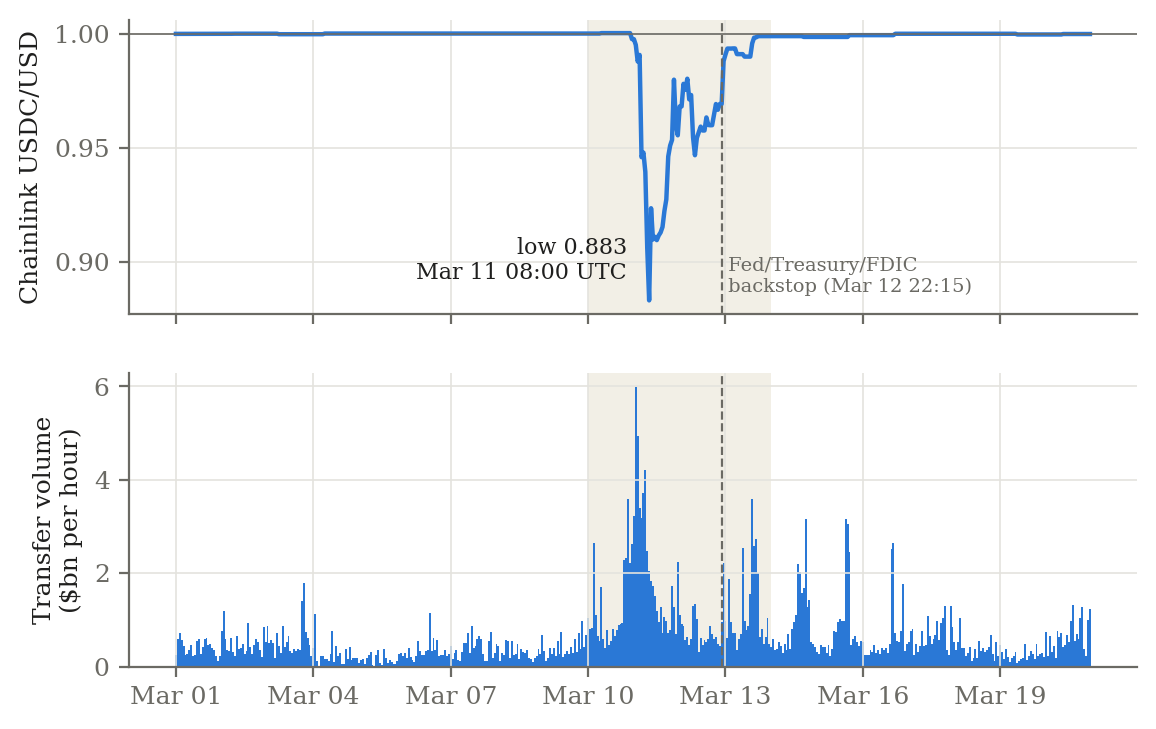
\includegraphics[width=0.9\textwidth]{fig1_price_volume.png}
\caption{USDC price and on-chain transfer volume. Top: Chainlink USDC/USD oracle price, read hourly from the chain. Bottom: hourly transfer volume excluding mints and burns. The shaded area is the stress window (March 10--13); the dashed line marks the joint Fed/Treasury/FDIC statement.}
\label{fig:price}
\end{figure}

Figure~\ref{fig:price} shows the episode. The oracle price falls below \$0.95 early on March 11 (UTC), bottoms at \$0.883 at 08:00 UTC, and recovers to about \$0.99 within an hour of the government backstop. Transfer volume spikes before the price trough: activity on March 10--11 is three to six times its pre-event level. Table~\ref{tab:periods} summarizes. During the stress window, daily transfers rose from 74,000 to 179,000, daily volume from \$9.8 billion to \$34.2 billion, and daily active addresses roughly doubled.

\begin{table}[t]
\centering\small
\caption{Activity by period. Daily averages of transfers, volume and active addresses; totals for mints, burns and net inflows into verified venues (positive = USDC flows into the venue).}
\label{tab:periods}
\begin{tabular}{lrrr}
\toprule
 & Pre (Mar 1--9) & Stress (Mar 10--13) & Post (Mar 14--20) \\
\midrule
Days & 9.00 & 4.00 & 7.00 \\
Transfers / day & 74,383 & 178,728 & 75,910 \\
Volume / day (\$bn) & 9.82 & 34.21 & 15.78 \\
Active addresses / day & 35,669 & 70,196 & 32,148 \\
Minted (\$bn) & 4.31 & 1.61 & 0.37 \\
Burned (\$bn) & 3.02 & 5.20 & 4.02 \\
Net to Maker PSM (\$bn) & -0.10 & 2.07 & -0.85 \\
Net to Curve 3pool (\$bn) & -0.03 & 0.02 & 0.02 \\
Net to Uniswap pools (\$bn) & -0.12 & 0.05 & -0.00 \\
Net to Aave/Compound (\$bn) & 0.24 & -0.35 & 0.06 \\
Net to Labeled CEX wallets (\$bn) & -0.08 & 0.01 & -0.16 \\
\bottomrule

\end{tabular}
\end{table}

\paragraph{The primary market.} Figure~\ref{fig:mintburn} plots daily issuance and redemption. Burns totaled \$5.2 billion during the stress window and another \$4.0 billion in the following week, while issuance fell to almost zero on Saturday and Sunday (\$0.06 and \$0.02 billion). Over the full sample, USDC supply on Ethereum fell by \$5.9 billion. Redemption was concentrated on March 10 (\$1.9 billion) and Monday, March 13 (\$1.7 billion), when the banking system reopened.

\begin{figure}[t]
\centering
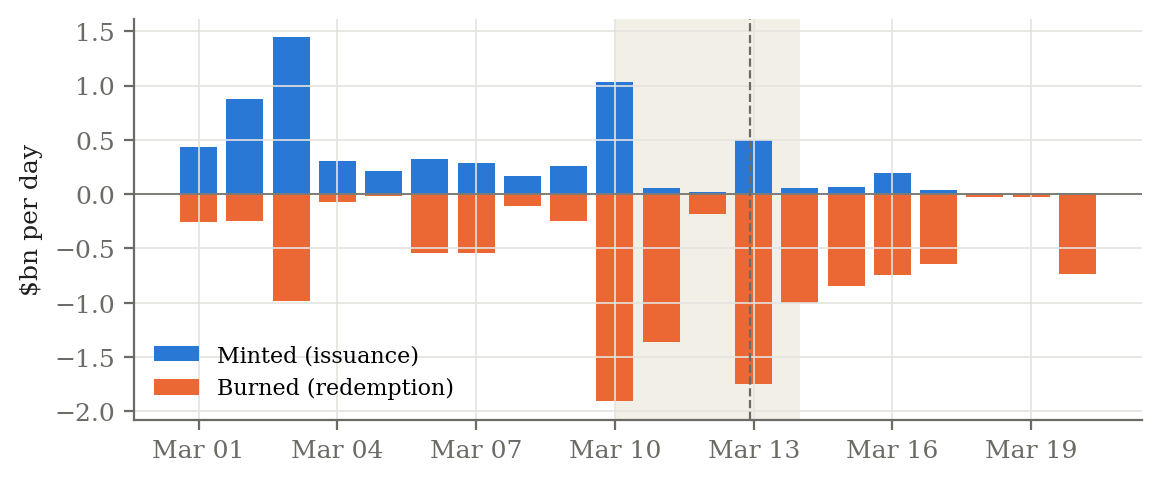
\includegraphics[width=0.9\textwidth]{fig2_mint_burn.png}
\caption{Daily USDC issuance (mints) and redemptions (burns) on Ethereum.}
\label{fig:mintburn}
\end{figure}

\paragraph{Where the selling went.} Figure~\ref{fig:venues} tracks cumulative net inflows into verified venues. The dominant on-chain exit route was MakerDAO's Peg Stability Module, which allowed USDC to be exchanged for DAI at a fixed rate: it absorbed \$2.1 billion of net inflow during the stress window, in two discrete steps on March 11, and gave back \$0.9 billion the following week as the peg was restored. Net flows into AMM pools were small in dollar terms because pools rebalance through price: USDC sold into a pool is largely offset by arbitrage flows.

\begin{figure}[t]
\centering
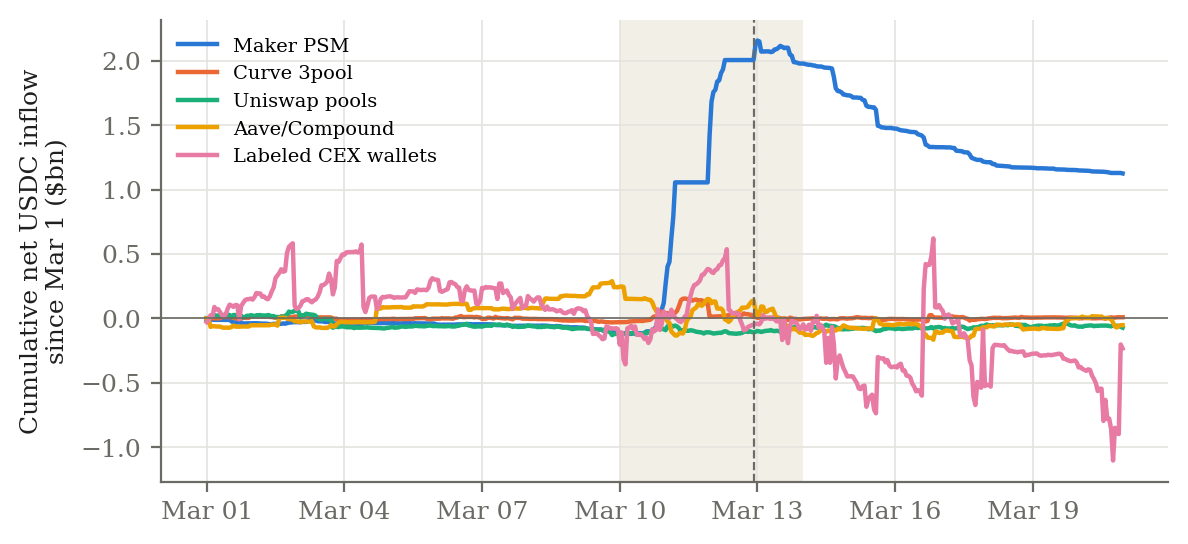
\includegraphics[width=0.9\textwidth]{fig3_venue_flows.png}
\caption{Cumulative net USDC inflow into verified venues since March 1. The CEX series uses unverified Etherscan tags for seven hot wallets.}
\label{fig:venues}
\end{figure}

\paragraph{Concentration.} Figure~\ref{fig:conc} reports the share of each day's outgoing volume (from addresses that are not labeled protocols) accounted for by the largest senders. On a normal day the top 100 senders account for 80--90\% of volume. On March 11 this share fell to 48\% and the number of distinct senders rose to over 95,000, roughly four times the usual level. The run broadened participation: activity spread across many wallets that ordinarily do not trade.

\begin{figure}[t]
\centering
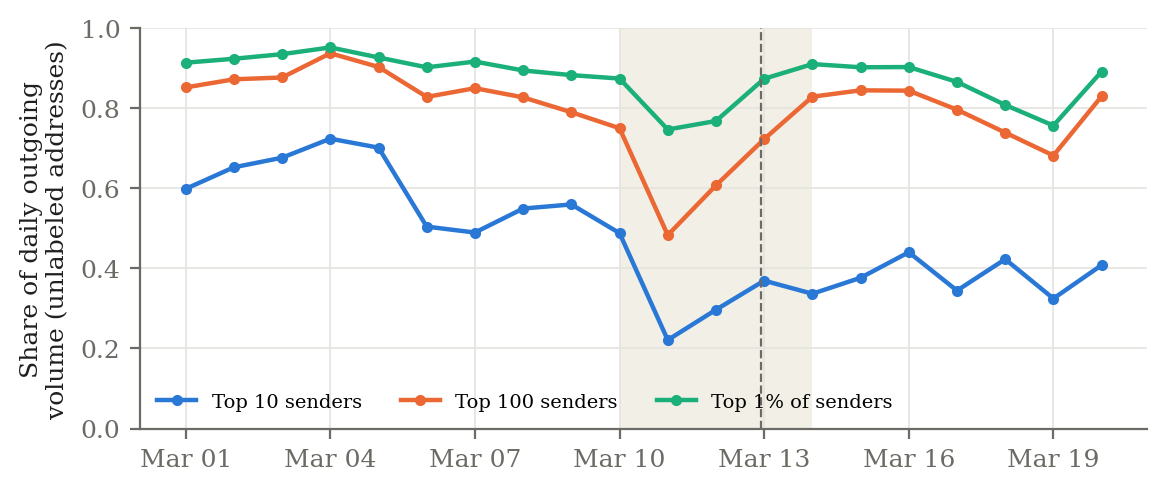
\includegraphics[width=0.9\textwidth]{fig4_concentration.png}
\caption{Concentration of daily outgoing USDC volume among non-protocol senders.}
\label{fig:conc}
\end{figure}

\section{Who Ran? Wallet-Level Evidence}

\paragraph{Outcomes.} For wallet $i$ and window $w \in \{\text{placebo}, \text{stress}\}$, both covering Friday to Monday (March 3--6 and March 10--13), define
\[
\text{NetOut}_{iw} = \frac{\text{Outflow}_{iw} - \text{Inflow}_{iw}}{\text{Balance}_{i,\text{start}(w)}},
\]
bounded above by one and capped at $-1$ from below. $\text{Ran}_{iw} = \mathbf{1}[\text{NetOut}_{iw} \ge 0.5]$ is an extensive-margin indicator, and $\text{Swap}_{iw}$ is the outflow sent directly into AMM pools, Curve or the PSM, scaled by the starting balance.

\paragraph{Specification.} With wallet fixed effects and two windows, the difference-in-differences regression
\[
Y_{iw} = \alpha_i + \gamma\,\text{Stress}_w + \sum_{g} \beta_g\,(\text{Size}_{g,i} \times \text{Stress}_w) + \varepsilon_{iw}
\]
is estimated in first differences, $\Delta Y_i = \gamma + \sum_g \beta_g \text{Size}_{g,i} + \delta\,\text{Contract}_i + u_i$, with heteroskedasticity-robust standard errors. The omitted group is \$1k--\$10k. The placebo window absorbs wallet-specific turnover that would occur in any Friday-to-Monday period.

\begin{table}[t]
\centering\small
\caption{Mean outcomes by size group (March 3 balance) and window.}
\label{tab:means}
\begin{tabular}{lrrrrrrr}
\toprule
 & & \multicolumn{2}{c}{NetOut} & \multicolumn{2}{c}{Swap} & \multicolumn{2}{c}{Ran} \\
\cmidrule(lr){3-4}\cmidrule(lr){5-6}\cmidrule(lr){7-8}
Size group & N & Placebo & Stress & Placebo & Stress & Placebo & Stress \\
\midrule
\$1k-10k & 44,095 & -0.002 & 0.602 & 0.012 & 0.150 & 0.022 & 0.627 \\
\$10k-100k & 35,237 & 0.011 & 0.602 & 0.011 & 0.167 & 0.023 & 0.624 \\
\$100k-1m & 11,818 & 0.018 & 0.543 & 0.007 & 0.123 & 0.024 & 0.566 \\
\$1m-10m & 2,295 & 0.018 & 0.476 & 0.005 & 0.087 & 0.024 & 0.501 \\
\$10m+ & 261 & 0.027 & 0.322 & 0.008 & 0.036 & 0.034 & 0.360 \\
\bottomrule

\end{tabular}
\end{table}

\begin{table}[t]
\centering\small
\caption{Difference-in-differences by holder size. Dependent variable: stress minus placebo change in the outcome. Robust standard errors in parentheses; *, **, *** denote significance at 10\%, 5\%, 1\%.}
\label{tab:reg}
\begin{tabular}{lrrrrrr}
\toprule
 & \multicolumn{2}{c}{$\Delta$NetOut} & \multicolumn{2}{c}{$\Delta$Swap} & \multicolumn{2}{c}{$\Delta$Ran} \\
\cmidrule(lr){2-3}\cmidrule(lr){4-5}\cmidrule(lr){6-7}
 & (1) & (2) & (3) & (4) & (5) & (6) \\
\midrule
\$10k-100k & -0.008* & -0.007* & 0.020*** & 0.021*** & 0.002 & 0.003 \\
 & (0.004) & (0.004) & (0.003) & (0.003) & (0.004) & (0.004) \\
\$100k-1m & -0.050*** & -0.058*** & -0.013*** & -0.014*** & -0.034*** & -0.043*** \\
 & (0.006) & (0.006) & (0.003) & (0.004) & (0.005) & (0.006) \\
\$1m-10m & -0.075*** & -0.102*** & -0.034*** & -0.043*** & -0.060*** & -0.085*** \\
 & (0.012) & (0.013) & (0.006) & (0.007) & (0.011) & (0.013) \\
\$10m+ & -0.177*** & -0.246*** & -0.070*** & -0.107*** & -0.152*** & -0.183*** \\
 & (0.033) & (0.047) & (0.009) & (0.013) & (0.031) & (0.043) \\
\midrule
Constant (\$1k-10k) & 0.611 & 0.613 & 0.140 & 0.140 & 0.612 & 0.613 \\
Contract control & Yes & -- & Yes & -- & Yes & -- \\
Sample & All & EOA & All & EOA & All & EOA \\
Observations & 93,706 & 89,528 & 93,706 & 89,528 & 93,706 & 89,528 \\
\bottomrule

\end{tabular}
\end{table}

\paragraph{Results.} Tables~\ref{tab:means} and~\ref{tab:reg} show a sharp and monotone pattern. In the placebo window, net outflows are close to zero for every group, and only 2--3\% of wallets move out half their balance. In the stress window, 63\% of \$1k--\$10k wallets do so, compared with 50\% of \$1m--\$10m wallets and 36\% of wallets above \$10 million. Relative to the smallest group, the largest holders' net-outflow share rose by 18 percentage points less (25 points less among EOAs), and their direct swap share by 7--11 points less. Contracts, which are more prevalent among large holders (2\% of the smallest group, 40\% of the largest), ran substantially less than EOAs of the same size.

\paragraph{Timing.} Figure~\ref{fig:timing} aggregates net outflows by size group within the stress window. Groups between \$10k and \$10m moved out roughly half of their combined March 10 balance, most of it between 18:00 UTC on March 10 and noon on March 11, so the bulk of the outflow happened \emph{before} the price trough. The largest holders moved out only about 7\% of their aggregate balance. I do not find that large holders moved earlier; rather, they largely did not move on-chain at all.

\begin{figure}[t]
\centering
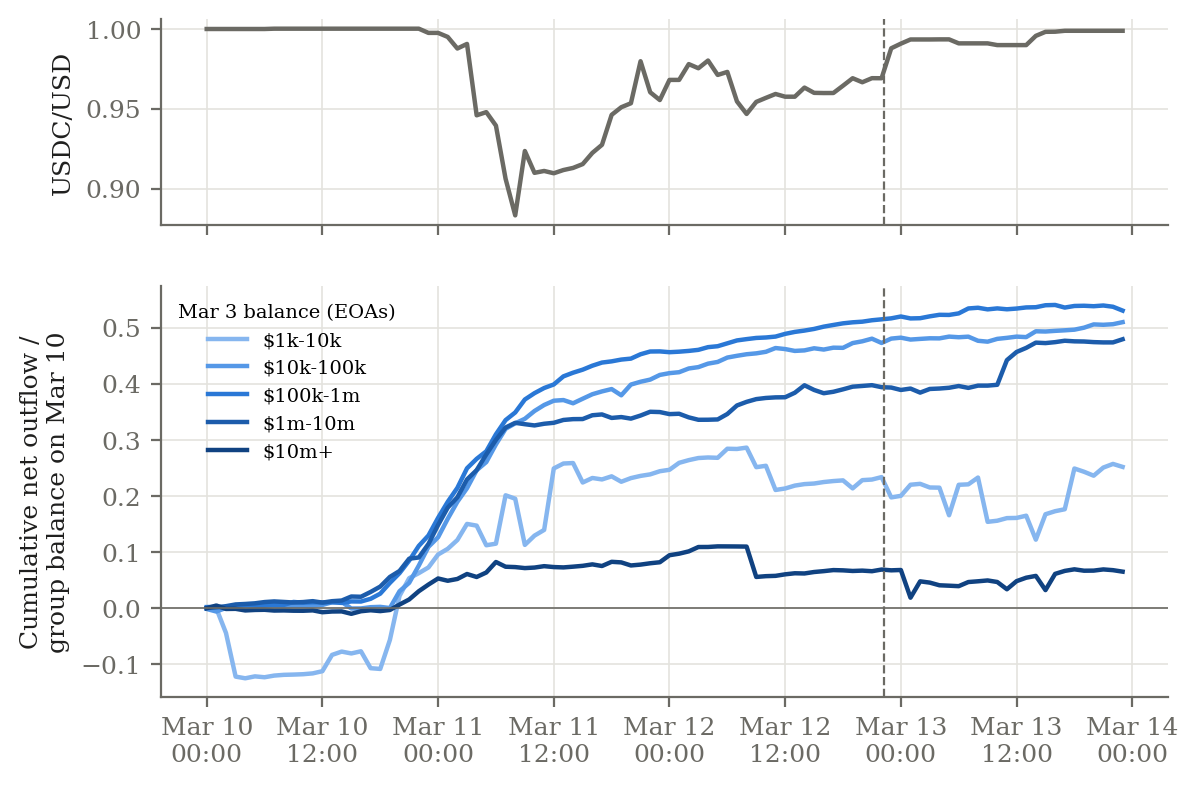
\includegraphics[width=0.9\textwidth]{fig5_timing_by_size.png}
\caption{Cumulative net outflow of EOA wallets during the stress window, by March 3 balance group, scaled by the group's aggregate balance on March 10. Top panel: oracle price.}
\label{fig:timing}
\end{figure}

\section{Interpretation and Limitations}

One reading of these patterns is that run behavior depends on access to the primary market. Large holders, often institutions with Circle accounts, could wait to redeem at par once banks reopened; the burn spike on Monday, March 13 is consistent with this. Small holders had no such option and sold on-chain at a discount, through the PSM, AMM pools and aggregators. This links to models in which redemption is restricted to a few arbitrageurs \citep{ma2023stablecoin}, and suggests a testable prediction: the wallets that ran are less likely to be linked, through transfer paths, to addresses that receive USDC from Circle's mint.

The evidence is descriptive and has clear limitations. (i) An address is not an investor: one entity can control many addresses, and exchange deposit addresses pool many users. A large share of outflows (56--73\% by group) goes to unclassified addresses, which may include users' own other wallets. (ii) Net outflow is not the same as a sale; it measures balance reallocation. (iii) The sample conditions on activity in the March 1--20 window, which overweights active traders. (iv) Exchange hot-wallet labels come from public tags and are not verified. The natural next steps are transaction-path tracing to classify the economic purpose of each outflow, linking wallets to Circle's mint and burn addresses to measure primary-market access, and extending the window to compare the experience of other stablecoins.

\paragraph{Reproducibility.} The repository contains every step from raw RPC calls to tables: \texttt{fetch\_transfers.py}, \texttt{build\_transfers.py} (validation), \texttt{fetch\_price.py}, \texttt{fetch\_balances.py}, \texttt{fetch\_codes.py}, \texttt{verify\_labels.py}, \texttt{classify\_counterparties.py}, and \texttt{analysis.py}. A full run takes about 30 minutes on a free public RPC endpoint.

\bibliographystyle{plainnat}
\begin{thebibliography}{9}
\bibitem[Liu et~al.(2023)]{liu2023anatomy}
Liu, J., I.~Makarov, and A.~Schoar (2023). Anatomy of a run: The Terra Luna crash. NBER Working Paper 31160.
\bibitem[Lyons and Viswanath-Natraj(2023)]{lyons2023stablecoins}
Lyons, R.~K. and G.~Viswanath-Natraj (2023). What keeps stablecoins stable? \emph{Journal of International Money and Finance} 131, 102777.
\bibitem[Ma et~al.(2023)]{ma2023stablecoin}
Ma, Y., Y.~Zeng, and A.~L. Zhang (2023). Stablecoin runs and the centralization of arbitrage. Working paper.
\bibitem[Makarov and Schoar(2020)]{makarov2020trading}
Makarov, I. and A.~Schoar (2020). Trading and arbitrage in cryptocurrency markets. \emph{Journal of Financial Economics} 135(2), 293--319.
\bibitem[Makarov and Schoar(2021)]{makarov2021blockchain}
Makarov, I. and A.~Schoar (2021). Blockchain analysis of the Bitcoin market. NBER Working Paper 29396.
\end{thebibliography}

\end{document}
